\section{Application to Model Selection for Primal SVM}

\textcolor{red}{Skalarprodukt anpassen, Vektoren nicht fett oder neue definition, notation, \(\lambda \in \Lambda\) einfugen}

\subsection{Introduction}

In this part of the thesis the nonconvex inexact bundle algorithm is applied to the problem of model selection for \emph{support vector machines} (SVMs) solving classification tasks.
It relies on a bilevel formulation proposed by Kunapuli in \cite{Kunapuli2008} and Moore et al. in \cite{Moore2011}.

A natural application for the inexact bundle algorithm is an optimization problem where the objective function value can only be computed iteratively. This is for example the case in bilevel optimization.
%If this objective function is iteratively optimized, the function value i never exact. But by the stopping condition it is (often???) possible to have the needed error bound on the function value (what about the gradient???). (Comment on asymptotical exactness?)

%A general bilevel problem can be formulated as 
%Bilevel optimization deals with a class of constrained optimization problems where one or more of the optimization variables are again constrained by optimization problems.
A general bilevel program can be formulated as in \cite[p. 20]{Kunapuli2008}

\begin{equation}
	\begin{array}{cll}
	\displaystyle\min_{x \in X, y} & F(x,y) & \text{upper level} \vspace{0.5ex}\\
	\text{s.t.} & G(x,y) \leq 0 & \vspace{1em}\\
	& y \in \begin{Bmatrix} \displaystyle\argmax_{y\in Y} & f(x,y) \vspace{0.5ex}\\
	                        \text{s.t.} & g(x,y) \leq 0 
													\end{Bmatrix}. & \text{lower level}
	\end{array}
\end{equation}

It consists of an \emph{upper} or \emph{outer level} which is the overall function to be optimized. Contrary to usual constrained optimization problems which are constrained by explicitly given equalities and inequalities a  bilevel program is additionally constrained by a second optimization problem, the \emph{lower} or \emph{inner level} problem.

Solving bilevel problems can be divided roughly in two classes: implicit and explicit solution methods. 
In the explicit methods the lower level problem is usually rewritten by its KKT conditions, these are then added as constraints to the upper level problem. With this solution method the upper and lower level are solved simultaneously. For the setting of model selection for support vector machines as it is used here, this method is described in detail in \cite{Kunapuli2008}.

The second approach is the implicit one. Here the lower level problem is solved directly in every iteration of the outer optimization algorithm and the solution is plugged into the upper level objective. 

Obviously if the inner level problem is solved numerically, the solution cannot be exact. Additionally the \emph{solution map} \( S(x) = \{y \in \R^k \mid y\), that solves the lower level problem, is can be nondifferentiable \cite{Outrata1998} and since elements of  the solution map are plugged into the outer level objective function in the implicit approach, the outer level function then becomes nonsmooth itself.This is why the inexact bundle algorithm seems a natural choice to tackle these bilevel problems. 

Moore et al. use the implicit approach in \cite{Moore2011} for support vector regression. However they use a gradient decent method which is not guaranteed to stop at an optimal solution.
In \cite{Moore2010a} he also suggests the nonconvex exact bundle algorithm of Fuduli et al. \cite{Fuduli2004a} for solving the bilevel regression problem. This allows for nonsmooth inner problems and can theoretically solve some of the issues of the gradient descent method. It ignores however, that the objective function values can only be calculated approximately. A fact which is not addressed in Fuduli's algorithm.

%\subsection{Notation and Expressions}

%training set, validation /holdout set...

\subsection{Introduction to Support Vector Machines}
%In times of big data machine learning is a very active field of research. 
Support vector machines are linear learning machines that were developed in the 1990's by Vapnik and co-workers. Soon they could outperform several other programs in this area \cite{Cristianini2000} and the subsequent interest in SVMs lead to a very versatile application of these machines \cite{Kunapuli2008}.

The case that is considered here is binary support vector classification using supervised learning. 
For a throughout introduction to this subject see also \cite{Cristianini2000}. Here a summary of the most important expressions and results is given.

In classification data from a possibly high dimensional vector space \(\tilde{X} \subset \R^n\), the \emph{feature} or \emph{input space} is divided into two classes. These lie in the \emph{output domain} \(\tilde{Y} = \{-1,1\}\). Elements from the feature space will mostly be called \emph{data points} here. They get \emph{labels} from the feature space. Labeled data points are called \emph{examples}.
The functional relation between the features and the class of an example is given by the usually unknown \emph{response} or \emph{target function} \(f(x)\).
Supervised learning is a kind of machine learning task where the machine is given examples of input data with associated labels, the so called \emph{training data} \((X,Y)\). Mathematically this can be modeled by assuming that the examples are  drawn identically and independently distributed (iid) from the fixed joint distribution \(P(x,y)\). This usually unknown distribution states the probability that a data point \(x\) has the label \(y\) \cite[p. 988]{Vapnik1999}.
The overall goal is then to optimize the generalization ability, meaning the ability to predict the output for unseen data correctly \cite[chapter 1.2]{Cristianini2000}.
%The overall goal of machine learning is to optimize the generalization ability of the algorithm --> this means: predict output for unlabeled input as well as possible.
%task is to find a mapping that predicts the output given unlabeled input as good as possible \cite{Cristianini2000}. 

\subsubsection{Risk minimization}
The concept of SVM's was originally inspired by the statistical learning theory developed by Vapnik. A detailed examination of the subject is given in \cite{Vapnik1998}. In \cite{Vapnik2013} the subject is approached from a more explaining point of view.

%from: Vapnik - Statistical Learning Theory overview \cite{Vapnik1998}
The idea of \emph{risk minimization} is to find from a fixed set or class of functions the one that is the best approximation to the response function. This is done by minimizing a loss function that compares the given labels of the examples to the response of the learning machine.
%goal: find best available (from set of functions that was chosen before) approximation to the actual (unknown) ``response function'' --> function that ``classifies'' the data
%Minimize loss between response of ``supervisor'' and response of learning machine

As the response function is not known only the expected value of the loss can be calculated. It is given by the \emph{risk functional} 

\begin{equation}
	R(\lambda) = \int{\mathcal{L}(y,f_{\lambda}(x))\text{d}P(x,y)}.
\label{risk_func}
\end{equation}

Here \(\mathcal{L}: \R^2 \to \R\) is the loss function, \(f_{\lambda}: \R^{n}\cap\mathcal{F} \to \R, ~ \lambda \in \Lambda\) the approximate response function found by the learning machine and \(P(x,y)\) the joint distribution the training data is drawn from. The goal is now to find a function \(f_{\bar{\lambda}}(x)\) in the chosen function space \(\mathcal{F}\) that minimizes this risk functional \cite[989]{Vapnik1999}.

As the only given information is provided by the training set inductive principles are used to work with the \emph{empirical risk}, rather than with the risk functional.
The empirical risk only depends on the finite training set  and is given by 

%goal: find \(f_{\lambda_0}(x)\) that minimizes this functional
%\(P(x,y)\) is unknown
%Because only a data sample is known: Work with the empirical risk

\begin{equation}
	R_{\text{emp}}(\lambda) = \frac{1}{l} \sum_{i = 1}^{l}\mathcal{L}(y_i,f_{\lambda}(x^i)),
\label{emp_risk}
\end{equation}

where \(l\) is the number of data points.
%L: Loss function 
%Goal: approximate \(Q(z,\lambda_0)\) by \(Q(z,\lambda_l)\) that minimizes the empirical risk. --> is called ERM (empirical risk minimization induction principle)
The law of large numbers ensures that the empirical risk converges to the risk functional as the number of data points grows to infinity. This however does not guarantee that the function \(f_{\lambda,\text{emp}}\) that minimizes the empirical risk also converges towards the function \(f_{\bar{\lambda}}\) that minimizes the risk functional.
The theory of consistency provides necessary and sufficient conditions that solve this issue  \cite[p. 989]{Vapnik1999}.

Vapnik therefore introduced the structural risk minimization (SRM) induction principle . It ensures that the used set of functions has a structure that makes it strongly consistent \cite{Vapnik1999}. Additionally it takes the complexity of the function that is used to approximate the target function into account. ``The SRM principle actually suggests a tradeoff between the quality of the approximation and the complexity of the approximating function'' \cite[p. 994]{Vapnik1999}.
This reduces the risk of \emph{overfitting}, meaning to overly fit the function to the training data with the result of poor generalization \cite[chapter 1.3]{Cristianini2000}.

%Therefore: structural risk Minimization induction Principle (SRM) --> is strongly consistent --> idea: minimize the empirical risk by considering the complexity of the model (given by CV-dimension)

Support vector machines fulfill all conditions of the SRM principle. Due to the kernel trick that allows for nonlinear classification tasks it is also very powerful. For more detailed information on this see \cite{Kunapuli2008} and references therein.

\subsubsection{Support Vector machines}

In the case of linear binary classification one searches for a an affine hyperplane \(w \in \R^n\) shifted by \(b \in \R\) to separate the given data. The vector \(w\) is called weight vector and \(b\) is the bias.

Let the data be linearly separable. The function deciding how the data is classified can then be written as

\[ f(x) = \text{sign}(\Langle w,x\Rangle-b). \]

Support vector machines aim at finding such a hyperplane that separates also unseen data optimally.

\textcolor{red}{???Picture of hyperplane}

One problem of this intuitive approach is that the representation of a hyperplane is not unique. If the plane described by \((w,b)\) separates the data, there exist infinitely many hyperplanes \((tw,b)\), \(t>0\), that separate the data in the same way.
To have a unique description of a separating hyperplane the \emph{canonical hyperplane for given data} \(x \in X\) is defined by 

\[ f(x) = \Langle w, x\Rangle - b  \quad \text{s.t.} \quad \min_i \vert\Langle w,x^i\Rangle -b\vert = 1.\] 

This is always possible in the case where the data is  linearly separable and means that the inverse of the norm of the weight vector is equal to the distance of the closest point \(x \in X \) to  the hyperplane \cite[p. 10]{Kunapuli2008}.


%Kunapuli: representation of hyperplane not unique --> if \((w,b)\) separates data, infinitely many hyperplanes \((tw,tb) \forall t > 0\) also separate data --> need unique representation --> w.l.o.g. define \emph{canonical hyperplane} for given data \(x \in X\) as function 
%only valid for separable data

This gives rise to the following definition:
The \emph{margin} is the minimal Euclidean distance between a training example \(x^i\) and the separating hyperplane.
%one can show that margin invese proportional to norm of \(w\).
A bigger margin means a lower complexity of the function \cite{Cristianini2000}. 

A \emph{maximal margin hyperplane} is the hyperplane that realizes the maximal possible margin for a given data set.

%Theorem 6.1
\begin{proposition}[{\cite[Proposition 6.1]{Cristianini2000}}]
Given a linearly separable training sample \ \(\Omega = \{(x^i,y_i),...,(x^l,y_l)\}\) the hyperplane \((w,b)\) that solves the optimization problem

\[\|w\|^2 \quad \text{s.t.} \quad y_i(\Langle w,x\Rangle-b)\geq 1, \quad i = 1,...,l, \]

realizes a maximal margin hyperplane.
\end{proposition}

The proof is given in \cite[chapter 6.1]{Cristianini2000}. 

Generally one cannot assume the data to be linearly separable. This is why in most applications a so called \emph{soft margin classifier} is used. It introduces the slack variables \(\xi_i\) that measure the distance of the misclassified points to the hyperplane:

%from this follows: soft margin classifyer --> not any more assumption that data linearly separable --> slack variables \(\xi_i\) measure the distance of misclassified points

%Def 2.6:
%\begin{definition} \cite{Cristianini2000}
Fix \(\gamma > 0\). A \emph{margin slack variable of the example} \((x^i,y_i)\) with respect to the hyperplane \((w,b)\) and target margin \(\gamma\) is 

\[\xi_i = \max(0, \gamma - y_i(\Langle w,x\Rangle+b))\] 

%\end{definition}  
If \(\xi_i > \gamma\) the point is considered misclassified. 
One can also say that \(\|\xi\|\) measures the amount by which training set ``fails to have margin \(\gamma\)'' \cite{Cristianini2000}.

For support vector machines the target margin is set to \(\gamma = 1\).

%Book uses \(\xi^2\) -> then \(\xi>0\) not needed any more; only \(\xi\) also used -> 1-norm
This results finally in the following slightly different
optimization problems for finding an optimal separating hyperplane \((w,b)\): 

\begin{align}
\begin{split}
	\min_{w,b,\xi} \quad & \frac{1}{2} \|w\|^2_2+C\sum_{i=1}^l{\xi_i} \\
	\text{s.t.} \quad & y_i(\Langle w,x^i\Rangle-b) \geq 1 - \xi_i \\
	& \xi_i \geq 0 \\
	& 	\forall i = 1, \dots , l
\end{split}
\label{SVM_1}
\end{align}

and

\begin{align}
	\min_{w,b,\xi} \quad & \frac{1}{2} \|w\|^2_2+C\sum_{i=1}^l{\xi_i^2} \vspace{0.5ex}\\
	\text{s.t.} \quad & y_i(\Langle w,x^i\Rangle-b) \geq 1 - \xi_i \vspace{0.5ex}\\
	& 	\forall i = 1, \dots , l.
\label{SVM_2}
\end{align}

The first part of the respective objective functions are the regularizations, the second part are the actual loss functions. 
The parameter \(C > 0\) gives a trade-off between the richness of the chosen set of functions \(f_{\lambda}\) to reduce the error on the training data and the danger of overfitting to have good generalization. It has to be chosen a priori \cite{Kunapuli2008}.
The two optimization problems only differ in the norm chosen for the loss function. In (\ref{SVM_1}) the one-norm is chosen, in (\ref{SVM_2}) the squared two-norm is used.
Problem (\ref{SVM_2}) is the one that is finally used in the bilevel approach where smoothness of the objective function of the inner level problem is needed to calculate all needed subgradients.

\subsection{Bilevel Approach and Inexact Bundle Method}
%Check if regression case also included?????

The hyper-parameter \(C\) in the objective function of the classification problem has to be set beforehand. This step is part of the model selection process.
To set this parameter optimally different methods can be used.
A very intuitive and widely used approach is doing  and \emph{cross validation} (CV) with a grid search implementation.
%very costly, discrete parameter choice, not practicable in case of many parameter

To prevent overfitting and get a good parameter selection, especially in case of little data, commonly \(T\)-fold cross validation is used.
For this technique the training data is randomly partitioned into \(T\) subsets of equal size. One of these subsets is then left out of the training set and instead used afterwards to get an estimate of the generalization error. 
To use CV for model selection it has to be embedded into an optimization algorithm over the hyper-parameter space. 
Commonly this is done by discretizing the parameter space and for \(T\)-fold CV training \(T\) models at each grid point. The resulting models are then compared to find the best parameters in the grid.
Obviously for a growing number of hyper-parameters this is very costly. An additional drawback is that the parameters are only chosen from a finite set \cite[p. 30]{Kunapuli2008}.

\subsubsection{Reformulation as Bilevel Problem}

A more recent approach is the formulation as a bilevel problem used in \cite{Kunapuli2008} and \cite{Moore2011}.
This makes it possible to optimize the hyper-parameters continuously.

%Formal description of the bilevel problem for t-fold cross validation
%Better model description --> see 2.2 (p.46) in thesis 

Let \(\Omega = \{(x^1,y_1),...,(x^l,y_l)\} \subset \R^{n+1}\) be a given data set of size \(l = |\Omega|\). The associated index set is denoted by \(\mathcal{N}\). For classification the labels \(y_i\) are \(\pm1\).
For \(T\)-fold cross validation let \(\bar{\Omega}_t\) and \(\Omega_t\) be the training set and the validation set respectively within the \(t\)'th fold and \(\bar{\mathcal{N}}_t\) and \(\mathcal{N}_t\) the respective index sets.
Furthermore let \(f^t:\R^{n+1}\cap\mathcal{F} \to \R\) be the response function trained on the \(t\)'th fold and \(\lambda \in \Lambda\) the hyper-parameters to be optimized.
For a general machine learning problem with upper and lower loss function \(\mathcal{L}_{upp}\) and \(\mathcal{L}_{low}\) respectively the bilevel problem reads
 
%%% introduce \mathcal(F) already before as the function space

\begin{equation}
	\begin{array}{cll}
	\displaystyle\min_{\lambda, f^t} & \mathcal{L}_{upp}\left(\lambda,f^1|_{\Omega_1},...,f^T|_{\Omega_T}\right) & \text{upper level} \vspace{0.5ex}\\
	\text{s.t.} & \lambda \in \Lambda & \vspace{1em}\\
	& \text{for } t = 1,...,T: & \\
	& f^t \in \begin{Bmatrix} \displaystyle\argmin_{f\in \mathcal{F}} & \mathcal{L}_{low}(\lambda,f,(x^i,y_i)_{i = 1}^l\in \bar{\Omega}_t) \vspace{0.5ex}\\
	                        \text{s.t.} & g_{low}(\lambda,f) \leq 0 
													\end{Bmatrix}. & \text{lower level}
	\end{array}
\end{equation}

In the case of support vector classification the \(T\) inner problems have the classical SVM formulation %(\ref{SVM_1}) or 
(\ref{SVM_2}). % (but all \(T\) problems have the same formulation).
The problem can also be rewritten into an unconstrained form. This form is helpful when using the inexact bundle algorithm for solving the bilevel problem.
For the \(t\)'th fold the resulting hyperplane is identified with the pair \((w^t,b_t) \in \R^{n+1}\).
The inner level problem for the \(t\)'th fold can therefore be stated as

%\begin{equation}
	%(w^t,b_t) \in \argmin_{w,b}\left\{ \frac{\lambda}{2} \|w\|^2_2+\sum_{i\in \bar{\mathcal{N}}_t}{\max\left(1-y_i(w^{\top}x^i-b),0\right)}\right\}
%\label{lower_t_1}
%\end{equation}

%or

\begin{equation}
	(w^t,b_t) \in \argmin_{w,b} \left\{\frac{\lambda}{2} \|w\|^2_2+\sum_{i\in \bar{\mathcal{N}}_t}{\max\left\{1-y_i\left(\Langle w,x^i\Rangle-b\right),0\right\}^2}\right\}
\label{lower_t_2}
\end{equation}

Where the hyper-parameter \(\lambda = \frac{1}{C}\) is used  due to numerical stability \cite[p. 38]{Kunapuli2008}.

For the upper level objective function there are different choices possible.
Simply put the outer level objective should compare the different inner level solutions and pick the best one. An intuitive choice is therefore to pick the misclassification loss, that counts how many data points of the respective validation set \(\Omega_t\) are misclassified when taking function \(f^t\).

The misclassification loss can be written as

\begin{equation}
	\mathcal{L}_{mis} = \frac{1}{T}\sum_{t=1}^T\frac{1}{|\mathcal{N}_t|}\sum_{i \in \mathcal{N}_t}{\left[-y_i\left(\Langle w^t,x^i\Rangle-b_t\right)\right]_{\star}},
\label{misclass_loss}
\end{equation}

where the step function \((\cdot)_{\star}\) is defined component wise for a vector as
\begin{equation}
	(r_{\star})_i = \left\{\begin{array}{c} 1, \quad \text{if } r_i > 0, \\ 0, \quad \text{if } r_i \leq 0 \end{array} \right. .
\label{step_fun}
\end{equation}

The drawback of this simple loss function is that it is not continuous and as such not suitable for subgradient based optimization. Therefore another loss function is used for the upper level problem - the \emph{hinge loss}. It is an upper bound on the misclassification loss and reads

\begin{equation}
		\mathcal{L}_{hinge} = \frac{1}{T}\sum_{t=1}^T\frac{1}{|\mathcal{N}_t|}\sum_{i \in \mathcal{N}_t}{\max\left(1-y_i\left(\Langle w^t,x^i\Rangle-b_t\right),0\right)}.
\label{hinge_loss}
\end{equation}

It is also possible to square the max term. This results in the loss function

\begin{equation}
		\mathcal{L}_{hinge} = \frac{1}{T}\sum_{t=1}^T\frac{1}{|\mathcal{N}_t|}\sum_{i \in \mathcal{N}_t}{\max\left\{1-y_i\left(\Langle w^t,x^i\Rangle-b_t\right),0\right\}^2}.
\label{hingequad_loss}
\end{equation}

In figure (\ref{??}) it can be seen that its minimum and overall progress is more similar to the misclassification loss than the one of the hinge loss. 
\textcolor{red}{For this reason we progress taking the squared form of the hinge loss, abbreviating with \emph{hingequad loss} for convenience.\\
No, take hingeloss because of nonsmoothness}

%\textcolor{red}{also possible to square the max term\\
%formula \\
%from plots: seems to match the misclassification loss a bit better -> used it instead/also}

Hence the final resulting bilevel formulation for model selection in support vector classification is 

%\begin{align}
%\begin{split}
	%\min_{w,\bm{b}} \quad &  \mathcal{L}_{hinge}(w,\bm{b}) = \frac{1}{T}\sum_{t=1}^T\frac{1}{|\mathcal{N}_t|}\sum_{i \in \mathcal{N}_t}{\max\left(1-y_i((w^t)^{\top}x-b_t),0\right)}\\
	%\text{subject to} \quad &  \lambda > 0 \\
	%& \text{for } t = 1,...,T \\
	%& (w^t,b_t) \in \argmin_{w,b}\left\{ \frac{\lambda}{2} \|w\|^2_2+\sum_{i\in \bar{\mathcal{N}}_t}{\max\left(1-y_i(w^{\top}x^i-b),0\right)}\right\} \\
%\end{split}
%\label{model_1}
%\end{align}
%
%and 

\begin{align}
\begin{split}
	\min_{w,b} \quad &  \mathcal{L}_{hinge}(w,b) = \frac{1}{T}\sum_{t=1}^T\frac{1}{|\mathcal{N}_t|}\sum_{i \in \mathcal{N}_t}{\max\left\{1-y_i\left(\Langle w^t,x^i\Rangle-b_t\right),0\right\}^2}\\
	\text{s.t.} \quad & \lambda > 0 \\
	& \text{for } t = 1,...,T \\
	& (w^t,b_t) \in \argmin_{w,b}\left\{ \frac{\lambda}{2} \|w\|^2_2+\sum_{i\in \bar{\mathcal{N}}_t}\max\left\{1-y_i\left(\Langle w,x^i\Rangle-b\right),0\right\}^2\right\}. \\
\end{split}
\label{model_2}
\end{align}


\subsubsection{Solution of the Bilevel Program}



\subsection{Numerical Experiments}

In this section algorithm \ref{sec_nonconv_inex}.1 is used to solve the bilevel problems presented above for different synthetic and real world data sets.

\begin{itemize}
	\item Problem what to optimize
	\item comment on nonlinear 
	\item overfitting
	\item pictures that show situation
\end{itemize}


\subsubsection{Selection of the Data Sets}

\begin{itemize}
	\item parameter \(\lambda\) against overfitting, there to make generalization better
	\item data sets that ``allow'' for high overfitting: not too big, many features
\end{itemize}

The following two real world data sets are used:

\begin{center}
\begin{table}[H]%
	\begin{tabular}{lcccc}
		\hline
    Data set & \(l_{train}\) & \(l_{test}\) & n & T \\
		\hline
		Wisconsin Breast Cancer Database & 240 & 443 & 9 & 3 \\
		John Hopkins University Ionosphere Database & 240 & 111 & 33 & 3
	\end{tabular}
	\caption{}
\end{table}
\end{center}


Plots

\begin{figure}[H]
	\begin{subfigure}{0.49\textwidth}
		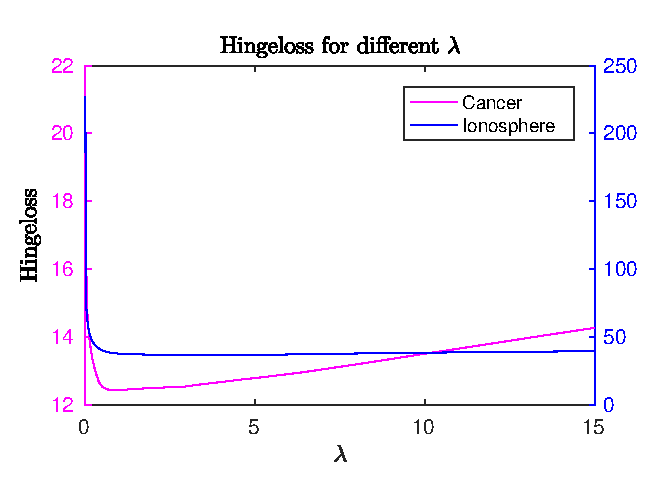
\includegraphics[width=\textwidth]{Pictures/Plots/lambda_vs_err_io_ca_final.eps}%
	\end{subfigure}
	\begin{subfigure}{0.49\textwidth}
		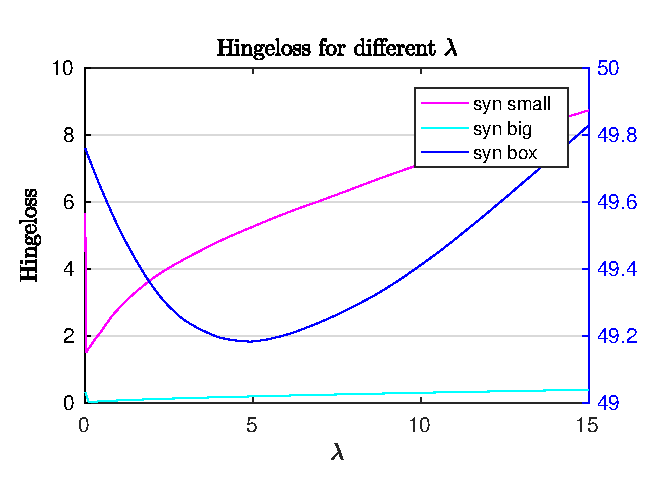
\includegraphics[width=\textwidth]{Pictures/Plots/lambda_vs_err_ss_sb_b5_final.eps}%
	\end{subfigure}
	\caption{Plots of the hingloss error for different $\lambda$ values. The figure on the right shows the plot for the \textup{\texttt{cancer}} (left axis) and \textup{\texttt{ionosphere}} (right axis) data sets. The blot on the left depicts the situation for the sythetic sets \textup{\texttt{syn small}}, \textup{\texttt{syn big}} (left axis) and \textup{\texttt{syn box}} (right axis).}%
	\label{fig_lambda_vs_err}%
\end{figure}


results

\begin{center}
\begin{table}[H]%
	\begin{tabular}{llcccc}
		\hline
    Data set & algorithm & 0.1 & 1 & 10 & 100 \\
		\hline
		\texttt{cancer} & Bundle & 1.0975 & 1.0974 & 1.0974 & 1.1341 \\
		 & Noll Bundle & 1.0974 & 1.0974 & 1.0974 & 1.0974 \\
		 &  fminsearch & 1.0974 & 1.0974 & 1.0974 & -10 \\
		 & fmindnb & 1.0974 \\
		\texttt{ionosphere} & Bundle & 2.6081 & 2.3108 & 0.3953 & 4.7401 \\
		 & Noll Bundle & 3.5386 & 3.6521 & 10 & 8.2773 \\
		 & fminsearch & 3.5104 & 3.5104 & 3.5104 & 3.5104 \\
		 & fminbnd & 3.5104 \\
		\texttt{syn small} & Bundle & 0.0337 & 0.031 & 0.0329& 0.03 \\
		 & Bundle Noll & 0.0323 & 0.0352 & 0.0352 & 0 \\
		 & fminsearch & 0.0346 & -0.1939 & -1.79 & -3.5673 \\
		 & fminbnd & 0.0346 \\
		\texttt{syn big} & Bundle & 0.1 & 1 & 10 & 100 \\
		 & Bundle Noll & 0.0099 & 0.0108 & 0.0109 & 0.0086 \\
		 & fminsearch & 0.0114 & -0.8748 & -0.8748 & -0.8748 \\
		 & fminbnd & 0.0206 & plot: 0.0114\\
		\texttt{syn box} & Bundle & 0.1 & 1 & 4.8486 & 4.45336 \\
		 & Bundle Noll & 0.1 & 1 & 4.2760 & 0 \\
		 & fminsearch & 4.8950 & 4.8950 & 4.8950 & 4.8950 \\
		 & fminbnd & 4.8950 \\
	\end{tabular}
	\caption{}
\end{table}
\end{center}

times

\begin{center}
\begin{table}[H]%
	\begin{tabular}{llcccc}
		\hline
    Data set & algorithm & 0.1 & 1 & 10 & 100 \\
		\hline
		\texttt{syn big} & Bundle Noll & 202 & 320 & 386 & 503 \\
		 & fminsearch & 672 & 637 & 587 & 741 \\
		 & fminbnd & 557
	\end{tabular}
	\caption{}
\end{table}
\end{center}

sometimes says problem not convex, then negative values. Why??? Because tries negative lambda values in course of optimization and then it gets negative \\
sometimes even for negative lambda in the end right solution \\
can I find out why bundle methods so bad? \\
try matlab method (smooth) with subgradient???



%%%%%%%%%%%%%%%%%%%%%%%%%%%%%%%%%%%%%%%%%%%%%%%%%%%%%%%%%%%%%%%%%%%%%%%%%%%%%%%%%%%%%%%%%%%%%%%%%%%%%%%%%%%%%%%%%%%%%%%%%%%%%%%%%%%%%%%%%

\subsubsection{Solution of the Bilevel Program}

\textcolor{red}{ab hier: Theorie fehlt\\
!!! notation - oder in prelininaries einfugen}
%ingredients for bundle method

To solve the given bilevel problem with the above presented nonconvex inexact bundle algorithm the algorithm jumps between the two levels. Once the inner level problems are solved for a given \(\lambda\) - this is possible with any QP-solver as the problems are convex - the bundle algorithm takes the outcome \(w\) and \(b\) and optimizes the hyper-parameter again.

The difficulty with this approach is that the bundle algorithm needs one subgradient of the outer level objective function with respect to the parameter \(\lambda\). However to compute this subgradient also one subgradient of \(w\) and \(b\) with respect to \(\lambda\) has to be known.

\textbf{The Differentiable Case}
\textcolor{red}{example in differentiable case}\\
Let us first assume that the outer and inner objective functions and \(w(\lambda)= \argmin \mathcal{L}_{low}(w,\lambda)\) are sufficiently often continuously differentiable to demonstrate the procedure of calculating the needed {(sub-)gradients}.

Let \(\mathcal{L}_{upp}(w,\lambda)\) be the objective function of the outer level problem, where the variable \(b\) was left out for the sake of simplicity.
To find an optimal hyper parameter \(\lambda\) given the input \(w\) the gradient \(g^{upp}_{\lambda}\) of \(\mathcal{L}_{upp}\) with respect to \(\lambda\) is needed in every iteration of the solving algorithm.
In order to calculate this gradient the chain rule is used yielding

\begin{equation*}
	g^{upp}_{\lambda} = \left(\frac{\partial}{\partial w}\mathcal{L}_{upp}(w,\lambda) \right)^{\top}\frac{\partial w(\lambda)}{\partial\lambda}+\frac{\partial}{\partial \lambda}\mathcal{L}_{upp}(w,\lambda).
\end{equation*}

The challenge is here to find the term \(\frac{\partial w(\lambda)}{\partial\lambda}\) because 

\[ \frac{\partial w}{\partial \lambda} \in \frac{\partial }{\partial \lambda} \argmin_{w} \mathcal{L}_{low}(w,\lambda). \]

Assuming \(\mathcal{L}_{low}\) is twice continuously differentiable at the  optimal solution \(w^*\) of the lower level problem the optimality condition for any parameter \(\lambda_0 > 0\)

\begin{equation}
	0 = \frac{\partial}{\partial w}\mathcal{L}_{low}(w^*,\lambda_0)
\label{opt_con}
\end{equation}


can be used to calculate the needed gradient in an indirect manner.

In the differentiable case the theoretical framework for the following calculations is given by the implicit function theorem.

\begin{theorem}[{c.f. \cite[chapter 3.4]{Koenigsberger2002}}]
	Let \(F: U \times V \to Z \), \(U\in\R^m, V,Z\in \R^n \), be a \(\mathcal{C}^1\) mapping, \((x_0,y_0) \in U\times V\)  and \(F(x_0,y_0) = 0\). If the matrix \(\frac{\partial}{\partial y}F(x_0,y_0)\) is invertible, there exist neighborhoods \(U_0\subset U\) of \(x_0\) and \(V_0\subset V\) of \(y_0\) and a continuously differentiable mapping \(f:U_0 \to V_0\) with 
	\begin{equation*}
	F(x,y) = 0, (x,y)\in U_0\times V_0  \quad \Leftrightarrow \quad y = f(x), x\in U_0.
	%\label{imp_fun_theo}
	\end{equation*}
\end{theorem}

Identifying \(x \estimates \lambda\), \(y \estimates w\) and  \(F(x_0,y_0) \estimates \frac{\partial}{\partial w} \mathcal{L}_{low}(w^*,\lambda_0)\) and assuming \(\frac{\partial^2 }{\partial  w^2}\mathcal{L}_{low}(w^*,\lambda_0)\) is invertible this theorem provides the existence of the continuously differentiable function \(w(\lambda)\) whose gradient is needed. \\
\textcolor{red}{what about the neighborhoods?}

If the inner level loss function yields a linear optimality condition in \(w\) it is possible to calculate the gradient explicitly. This is for example the case for SVM loss functions with a squared one- or two-norm as given in problem (\ref{SVM_2}).
The optimality condition can then be written as the linear system

\begin{equation*}
	H(\lambda)w = h(\lambda).
\end{equation*}

By taking the partial derivative with respect to \(\lambda\) on both sides of the system one gets

\begin{equation*}
	\frac{\partial H(\lambda)}{\partial \lambda}w+H(\lambda)\frac{\partial w}{\partial \lambda} = \frac{\partial h(\lambda)}{\partial  \lambda}.
\end{equation*}

If \(H(\lambda)\) is invertible for all \(\lambda \in \Lambda\) then the needed gradient is given by 

\begin{equation*}
	\frac{\partial w}{\partial \lambda} = H^{-1}(\lambda)\left(\frac{\partial h(\lambda)}{\partial \lambda}-\frac{\partial H(\lambda)}{\partial \lambda}w\right).
\end{equation*}

%\textcolor{red}{why H invertible??? - because we assume existence of \(w\)???}\\

\textbf{The Nondifferentiable Case}
\textcolor{red}{now for subgradients}

In practice we cannot expect \(\mathcal{L}_{low}\) to satisfy such strong differentiability properties.
It is therefore only assumed that \(\mathcal{L}_{low}\) is once continuously differentiable in \(w\). This assures that the optimality condition of the lower level problem is an equality like in (\ref{opt_con}).
%If \(\mathcal{L}_{low}\) was only locally Lipschitz the optimality condition states that zero is part of the subgradient set  \(\partial \mathcal{L}_{low}(w^*,\lambda_0)\).  
Contrary to the exemplary calculations from above in practice the second derivative \(\frac{\partial^2}{\partial w \partial \lambda} \mathcal{L}_{low}(w(\lambda),\lambda)\) however is not existent in this form, but a set of subgradients.



\textcolor{red}{\textbf{Notation}}\\
First the theoretical framework given to derive the results from above in the nondifferentiable case



\textcolor{red}{An important result about Lipschitz functions is Rademacher's theorem which states that these functions are differentiable almost everywhere but on a set of Lebesgue measure zero\cite[Theorem 3.1]{Heinonen2004}. 
Clarke deduces from this that the subdifferential at each of the nondifferentiable points is the convex hull of the limits of the sequence gradients a these points \cite[see Theorem 2.5.1]{Clarke1990}.}

This motivates the multidimensional definition of Clake's generalized gradient 

\textcolor{red}{
\begin{definition}[{\cite[Definition 2.6.1]{Clarke1990}}]
	\emph{generalized Jacobian}: \(F:\R^n \to \R^m\), with locally Lipschitz component functions \(F(x) = (f_1(x),...,f_m(x))\).\\
	Denote generalized Jacobian by \(\partial F(x) = conv\left(\lim JF(x_i)|x_i\to x, x_i \notin \Omega_F \right) \) where \(\Omega_F\) is the set of nondifferentiable points of \(F\)
\end{definition}
(after that comes proposition with properties of \(\partial F\))}


\textcolor{red}{To facilitate readability we use the following notation for the derivation of the nondifferentiable results.}

The \emph{'partial' subdifferential} of a function \(f(a^*,b_0,c_0,...)\) at the point \(a^*\) with respect to one variable \(a\) when all other variables are fixed is denoted by 
\begin{equation*}
	\partial^{a} f(a^*,b_0,c_0,...).
\end{equation*}

A subgradient of this subdifferential is written \(g^{a} \in \partial^{a} f(a^*,b_0,c_0,...)\).

Next step: show that chain rule is still valid in the nonsmooth case
Chain rules for subdifferential \\

\begin{theorem}[{\cite[Theorem 2.6.6]{Clarke1990}}]
	Let \(f(x)=\phi(F(x))\), with the locally Lipschitz functions \(F: \R^n \to \R^m\) and \(\phi:\R^m \to \R\). Then \(f\) is locally Lipschitz and it holds
	\begin{equation*}
		\partial f \subset \text{conv}\left\{\partial \phi(F(x))\partial F(x)\right\}.
	\end{equation*}
	If in addition \(\phi\) is strictly differentiable at \(F(x)\), then equality holds.
\end{theorem}

\textcolor{red}{strictly differentiable: c.f. \cite[Theorem 9.17 and 9.18]{Rockafellar2009} locally Lipschitz continuous and at most one subgradient at the point in question (see also comment to Definition 91 in \cite{Rockafellar2009})}

\begin{theorem}[c.f. {\cite[Theorem 7.1]{Rockafellar1985}}]
	Let \(p(x) = f(F(x))\), where \(F:\R^n \to \R^d\) is locally Lipschitz and \(f:\R^d \to \R\) is lower semicontinuous. 
	Assume \[\nexists y \in \partial^{\infty}f(F(\bar{x})), y \neq 0 \quad \text{with} \quad 0 \in y \partial F(\bar{x}). \]
	Then for the sets 
	\[ M(\bar{x}):= \partial f(F(\bar{x}))\partial F(\bar{x}), \quad M^{\infty}(\bar{x}):= \partial^{\infty}f(F(\bar{x}))\partial F(\bar{x}), \]
	one has \(\hat{\partial}p(\bar{x}) \subset M(\bar{x})\) and \(\hat{\partial}^{\infty} p(\bar{x}) \subset M^{\infty}(\bar{x})\).
\end{theorem}

The main idea is to replace the inner level problem by its optimality condition


\(\partial(w,b)\) means in this case that the subdifferential is taken with respect to the variables \(w\) and \(b\). \\
-> theory for subdifferentials in more than one variable!!! \\

For convex inner level problem this replacement is equivalent to the original problem.

The difference to the approach described in \cite{Kunapuli2008} is that the problem is not smoothly replaced by its KKT conditions but only by this optimality condition. The weight vector \(w\) and bias \(b\) are treated as a function of \(\lambda\) and are optimized separately from this hyper-parameter.
The reformulated bilevel problem becomes:

\begin{align}
	\begin{split}
	\min_{w,\bm{b}} \quad &  \mathcal{L}_{hinge}(w,\bm{b}) = \frac{1}{T}\sum_{t=1}^T\frac{1}{|\mathcal{N}_t|}\sum_{i \in \mathcal{N}_t}{\max\left(1-y_i((w^t)^{\top}x-b_t),0\right)}\\
	\text{subject to} \quad & \lambda > 0 \\
	& \text{for } t = 1,...,T \\
	& 0 \in \partial(w,b)\mathcal{L}_{low}(\lambda,w^t,b_t) \\
\end{split}
\label{SVM_opt_cond}
\end{align}

where \(\mathcal{L}_{low}\) can be the objective function of either of the two presented lower level problems.



solve the inner level problem (quadratic problem in constrained case) by some QP solver \\
put solution into upper level problem and solve it by using bundle method \\
difficulty: subgradient is needed to build model of the objective function --> need subgradient \(\frac{\partial \mathcal{L}}{\partial \lambda}\) --> for this need \(\frac{\partial (W,b)}{\partial \lambda}\) \\
but \((w,b)\) not available as functions -> only values

Moore et al. \cite{Moore2011} describe a method for getting the subgradient from the KKt-conditions of the lower level problem:

lower level problem convex -> therefore optimality conditions (some nonsmooth version -> source???) necessary and sufficient -> make ``subgradient'' of optimality conditions and then derive subgradient of w, b from this. \\
---> what are the conditions? optimality condition Lipschitz? 

Say (show) that all needed components are locally Lipschitz; state theorems about differentiability almost everywhere and convex hull of gradients gives set of subgradients\\
introduce special notation (only for this section) and because of readability adopt ``gradient writing''

Subgradients:
\(\mathcal{G}_{upp,\lambda}, \mathcal{G}_{upp,w},\mathcal{G}_{upp,b}\) -> subgradients of outer objective \\
\(g_w, g_b\) -> subgradient of w, b

\[ final subgradient = \left(\mathcal{G}_{upp,w}(w,b,\lambda)\right)^{\top}g_w+\left(\mathcal{G}_{upp,b}(w,b,\lambda)\right)^{\top}g_b+\mathcal{G}_{upp,\lambda}(w,b,\lambda) 
\label{subgr_upp}\]

subgradients \(\mathcal{G}_{upp,...}\) easy to find (assumption that locally Lipschitz) -> in this application differentiable

difficulty: find \(g_w, g_b\)
important: optimality condition must be a linear system in \(w,b\) -> this is the case in this application
\[ H(\lambda)\cdot (w,b)^{\top} = h(\lambda) \]

find subgradients of each element (from differentiation rules follows)

\[ \partial_{\lambda} H\cdot (w,b)^{\top} + H \cdot(\partial_{\lambda} w, \partial_{\lambda} b)^{\top} = \partial_{\lambda} h  \]

solve this for \((w,b)\):
\[ (\partial_{\lambda} w, \partial_{\lambda}b)^{\top} = H^{-1}\left(\partial_{\lambda}h-\partial_{\lambda} H \cdot(w,b)^{\top}\right) \]

matrix \(H\) has to be inverted -> in the feature space so scalable with size of data set -> still can be very costly \cite{Moore2011}

Applied to the two bilevel classification problems derived above, the subgradients have the following form:

derivative of upper level objective:
Notation: \(\delta_i := 1-y_i(w^{\top}x^i-b)\)

\begin{align}
	\partial_{w}\mathcal{L}_{upp}&= \frac{1}{T}\sum_{t=1}^T\frac{1}{\mathcal{N}_t}\sum_{i \in \mathcal{N}_t}{\left\{\begin{array}{cl} -y_ix^i & \text{if } \delta_i >0 \\ 0 & \text{if } \delta_i \leq 0 \end{array} \right.} \\
	\partial_{b}\mathcal{L}_{upp}&= \frac{1}{T}\sum_{t=1}^T\frac{1}{\mathcal{N}_t}\sum_{i \in \mathcal{N}_t}{\left\{\begin{array}{cl} y_i & \text{if } \delta_i >0 \\ 0 & \text{if } \delta_i \leq 0 \end{array} \right.}
	\end{align}
	
	here at the kink subgradient 0 is taken

for hingequad: -> here subgradient \\
optimality condition:
\begin{align}
	0 = \partial_{w}\mathcal{L}_{low} &= \lambda w+2\sum_{i \in \bar{\mathcal{N}_t}}{\left\{\begin{array}{cl} (1-y_i(w^{\top}x^i-b))(-y_ix^i) & \text{if } \delta_i >0 \\ 0 & \text{if } \delta_i \leq 0 \end{array} \right.} \\
	0 = \partial_b\mathcal{L}_{low} &= 2\sum_{i \in \bar{\mathcal{N}_t}}{\left\{\begin{array}{cl} (1-y_i(w^{\top}x^i-b))(y_i) & \text{if } \delta_i >0 \\ 0 & \text{if } \delta_i \leq 0 \end{array} \right.}
	\end{align}
	
subgradient??? is this smooth? with respect to \(\lambda\)
\begin{align}
	0 &= w+\lambda\partial_{\lambda}w+2\sum_{i \in \bar{\mathcal{N}_t}}{\left\{\begin{array}{cl} (-y_i(\partial_{\lambda}w^{\top}x^i-\partial_{\lambda}b))(-y_ix^i) & \text{if } \delta_i >0 \\ 0 & \text{if } \delta_i \leq 0 \end{array} \right.} \\
	0 &= 2\sum_{i \in \bar{\mathcal{N}_t}}{\left\{\begin{array}{cl} (-y_i(\partial_{\lambda}w^{\top}x^i-\partial_{\lambda}b))(y_i) & \text{if } \delta_i >0 \\ 0 & \text{if } \delta_i \leq 0 \end{array} \right.}
\end{align}

From this the needed subgradients can be calculated via:

\begin{equation}
	2\cdot\begin{pmatrix} \frac{\lambda}{2}+\sum_{i \in \bar{\mathcal{N}_t}}{y_i^2x^i(x^i)^{\top}} & \sum_{i \in \bar{\mathcal{N}_t}}	{-y_i^2x^i} \\ \sum_{i \in \bar{\mathcal{N}_t}}{-y_i^2(x^i)^{\top}} & \sum_{i \in \bar{\mathcal{N}_t}}{y_i^2}\end{pmatrix}
	\cdot \begin{pmatrix} \partial_{\lambda}w \\ \partial_{\lambda}b\end{pmatrix}
	= \begin{pmatrix}-w \\ 0\end{pmatrix}
\label{subgr_wb}
\end{equation}

for hinge not quad:

not as much information in the subgradient/derivative

similar calculation leads to 

\begin{align}
	\partial_{\lambda}w &= -\frac{w}{\lambda} \\
	\partial_{\lambda}b &= 0
\end{align}

\textcolor{red}{does not work with just Hingeloss because set valued optimality condition --> have to find ``corresponding'' equation to the chosen subgradient --> do not know how}

\subsubsection{Multi Group Model}

Idea: different samples within the group have different have different quality --> put the samples with similar quality within one group --> give it its own \(\lambda_g\) such that the groups are weighted depending on their quality.

two goals: better modleing and implicit information about the groups provided by the parameter \(\lambda_g\) -> small \(\lambda\) good quality, large \(\lambda\) bad quality???

Examle: different people do same experiment; measure same data...

\textbf{Model (Bilevel Problem)}


for simplicity: all groups of same size; in all folds same number of elements of each group

!! not possible to work with \(\lambda\) here, have to work with \(C\)-Formulation



\begin{align}
\begin{split}
	\min_{w,b} \quad &  \mathcal{L}_{hinge}(w,b) = \frac{1}{T}\sum_{t=1}^T\frac{1}{|\mathcal{N}_t|}\sum_{i \in \mathcal{N}_t}{\max\left\{1-y_i\left(\Langle w^t,x^i\Rangle-b_t\right),0\right\}}\\
	\text{s.t.} \quad & C = [C_1,...,C_G]^{\top} > 0 \text{ and} \\
	& \text{for } t = 1,...,T \\
	& (w^t,b_t) \in \argmin_{w,b}\left\{ \sum_{g = 1}^G \left(\frac{1}{2} \|w\|^2_2+C_g\sum_{i\in \bar{\mathcal{N}}_t^g}\max\left\{1-y_i\left(\Langle w,x^i\Rangle-b\right),0\right\}^2\right)\right\}. \\
\end{split}
\label{multi_group}
\end{align}


Reformulation of the lower level objective:

\begin{equation*}
	\mathcal{L}_{low}(w,b) =  \frac{1}{2} \|w\|^2+\sum_{g = 1}^GC_g\left(\sum_{i\in \bar{\mathcal{N}}_t^g}\max\left\{1-y_i\left(\Langle w,x^i\Rangle-b\right),0\right\}^2\right)
\label{ll_mult_group}
\end{equation*}

Reformulation for solution of lower level problem with \texttt{qudprog}:

\begin{align*}
	\min_{w,b,\xi} \quad & \frac{1}{2} \|w\|^2_2+\sum_{g = 1}^G\left(C_g\sum_{i \in \bar{\mathcal{N}}_t^g}{\xi_i^2}\right) \vspace{0.5ex}\\
	\text{s.t.} \quad & y_i\left(\Langle w,x^i\Rangle-b\right) \geq 1 - \xi_i \vspace{0.5ex}\\
	& 	\forall i \in \bigcup_{g =1}^G \bar{\mathcal{N}}_t^g = \bar{\mathcal{N}}_t
\label{MultiSVM_QP}
\end{align*}

the \(\mathcal{N}_t^g\) are pairwise disjoint

\(w \in \R^n, b\in \R, \xi \in \R^{\vert\bar{\mathcal{N}}_t \vert}\)

matrices for MATLAB calculations:

\begin{equation*}
\begin{split}
	& \frac{1}{2} \langle x,Hx \rangle + h \\
	& Ax \leq b
\end{split}
\end{equation*}

\begin{equation}
	H = \begin{pmatrix}
		\mathbb{I}_{n\times n} \\
		& 0 \\
		& & 2 C \\
	\end{pmatrix}
	\in \R^{feat+1+J\max\{T-1,1\}G\times feat+1+J\max\{T-1,1\}G}
\end{equation}

\[ h = 0, \qquad A = \begin{pmatrix} -YX^{\top} & Y & -\mathbb{I}_{J\max\{T-1,1\}G \times J\max\{T-1,1\}G} \\ \end{pmatrix},  \qquad b = -\mathtt{ones}(J\max\{T-1,1\}G,1) \] 

with \(C = [\underbrace{c_1,...,c_1}_{J\max\{T-1,1\} \text{ times}},c_2,...,c_2,...,c_G,...,c_G]^{\top}\).

\textbf{Derivatives}

overall gradient:
	\[ \frac{\textup{d}\mathcal{L}_{upp}}{\textup{d}\lambda} = {\underbrace{\frac{\partial \mathcal{L}_{upp}}{\partial (w,b)}}_{\in \R^{n+1}}} ^{\top} \underbrace{\frac{\partial (w,b)}{\partial \lambda}}_{\in \R^{n+1 \times G}} \in \R^G\]


gradient outer level objective: 
	\[ \frac{\partial \mathcal{L}_{upp}}{\partial w} = \frac{1}{T}\sum_{t=1}^T\frac{1}{|\mathcal{N}_t|}\sum_{i \in \mathcal{N}_t} \delta_i \left( -y_i x^i\right) \in \R^n\]
	
	\[ \frac{\partial \mathcal{L}_{upp}}{\partial b} = \frac{1}{T}\sum_{t=1}^T\frac{1}{|\mathcal{N}_t|}\sum_{i \in \mathcal{N}_t} \delta_i y_i \in \R\]
	
	\[ \delta_i = \left\{ \begin{array}{cl} 1 & \text{if } 1-y_i\left(\Langle w,x^i\Rangle-b\right) > 0 \\
		0 & \text{else}\end{array} \right.\]


in MATLAB: 
	\[ \frac{\partial \mathcal{L}_{upp}}{\partial w} = \frac{1}{T}\texttt{sum}(-\texttt{bsxfun}(\texttt{@times},X,\texttt{delta}.*Y) ,2) \in \R^n\]
	
	\[ \frac{\partial \mathcal{L}_{upp}}{\partial b} = \frac{1}{T}\texttt{sum}(\texttt{delta}.*Y ,1) \in \R\]
	
	
gradient lower level objective:\\
first optimality conditions \(0 = \frac{\partial \mathcal{L}_{low}}{\partial w}, 0 = \frac{\partial \mathcal{L}_{low}}{\partial b}\):
	\[ 0 = {\sum_{g = 1}^G(\lambda_g}w) + 2\sum_{i \in \bar{\mathcal{N}}_t}\delta_i \left\{1-y_i\left(\Langle w,x^i\Rangle -b\right) \right\}(-y_ix^i) \in \R^n \]
		
	\[0 = 2\sum_{i \in \bar{\mathcal{N}}_t}\delta_i \left\{1-y_i\left(\Langle w,x^i\Rangle -b\right) \right\}(y_i) \in \R \]
	
	derivatives with respect to \(\lambda_g, g = 1,...,G\), then \(\in \R^{n+1 \times G}\)
	
	write one column of the matrix \(\in \R^{n+1}\) \(\to\) \(G\) such columns:
	
	\[ 0 = w + \lambda_g\frac{\partial w}{\partial \lambda_g} + 2 \sum_{i \in  \bar{\mathcal{N}}_t} \delta_i \left(y_i^2x^i(x^i)^{\top}\frac{\partial w}{\partial \lambda_g} - y_i^2x^i \frac{\partial b}{\partial \lambda_g}\right) \in \R^n \]
	
	\[ 0 = 2\sum_{i \in  \bar{\mathcal{N}}_t} \delta_i \left(-y_i^2(x^i)^{\top} \frac{\partial w}{\partial \lambda_g} + y_i^2 \frac{\partial b}{\partial \lambda_g}\right) \in \R\] 


	rewrite to calculate \([\partial w / \partial \lambda, \partial b / \partial \lambda]^{\top} \in \R^{n+1 \times G}\) \(\to\) have to calculate every column of this matrix on its own \\
	solve \(G\) times this system of equations
	
	\[ 2\begin{pmatrix} \frac{\lambda_g}{2}\mathbb{I}+\sum_{i \in  \bar{\mathcal{N}}_t}{\delta_i(y_i^2x^i(x^i)^{\top})} &  \sum_{i \in  \bar{\mathcal{N}}_t} \delta_i (- y_i^2x^i )	\\
	\sum_{i \in  \bar{\mathcal{N}}_t} \delta_i (-y_i^2(x^i)^{\top}) & \sum_{i \in  \bar{\mathcal{N}}_t} \delta_i (y_i^2 )
	\end{pmatrix} 
	\begin{pmatrix}	\frac{\partial w}{\partial \lambda_g} \\ \frac{\partial b}{\partial \lambda_g}
	\end{pmatrix} 
	= \begin{pmatrix} -w \\ 0	\end{pmatrix} \]










